\chapter{Results}
\label{chapter:results}
\section{Model comparison}
\subsection{Stage one dataset}
\begin{table}[h]
    \centering
    \begin{tabular}{|l|c|c|c|c|c|c|}
        % Model                                 & $AP_{50}$ & $AP$    & $AP_{small}$ & $AP_{medium}$ & $AP_{large}$ & $AP_{75}$             \\\hline
        \hline
        Model                  & $AP$  & $AP@.5$ & $AP@.75$ & $AP@.5_S$ & $AP@.5_M$ & $AP@.5_L$ \\ \hline
        FRCNN-R50              & 0.045 & 0.168   & 0.0064   & 0.031     & 0.064     & 0.0058    \\ \hline
        YOLOv3                 & 0.093 & 0.258   & -        & -         & -         & -         \\ \hline
        YOLOv5-l6              & 0.097 & 0.318   & 0.03     & 0.211     & 0.309     & 0.0.397   \\ \hline
        YOLOv5-x6              & 0.105 & 0.337   & 0.05     & 0.204     & 0.324     & 0.413     \\ \hline
        EfficientDet-d4        & 0.101 & 0.298   & 0.02     & 0.215     & 0.404     & 0354      \\ \hline
        EfficientDet-d4, train & 0.421 & 0.839   & 0.362    & 0.251     & 0.501     & 0.535     \\ \hline
    \end{tabular}
    \caption{Comparision of trained model on the stage one dataset}
    \label{tab:model_results:stage_one}
\end{table}

\subsection{Stage two dataset}

\begin{table}[h]
    \centering
    \begin{tabular}{|l|c|c|c|c|c|c|}
        \hline
        Model                  & $AP$  & $AP@.5$ & $AP@.75$ & $AP@.5_S$ & $AP@.5_M$ & $AP@.5_L$ \\ \hline
        YOLOv3                 & 0.093 & 0.258   & -        & -         & -         & -         \\ \hline
        YOLOv5 L               & 0.097 & 0.318   & 0.03     & 0.904     & 0.12      & 0.05      \\ \hline
        YOLOv5 XL              & 0.105 & 0.337   & 0.05     & 0.986     & 0.133     & 0.11      \\ \hline
        EfficientDet d4        & 0.31  & 0.699   & 0.2054   & 0.215     & 0.404     & 0.47      \\ \hline
        EfficientDet d4, train & 0.421 & 0.839   & 0.362    & 0.251     & 0.501     & 0.535     \\ \hline
    \end{tabular}
    \caption{Comparision of trained model on the stage two dataset}
    \label{tab:model_results:stage_two}
\end{table}

\subsection{Stage three dataset}
Results of trained models evaluated on the training part and the test part of the dataset are available in tables \ref{tab:model_results:stage_three:train} and \ref{tab:model_results:stage_three:test}. Performance comparison of different YOLOv5 backbones can be seen in table \ref{tab:stage_three:yolov5_backbones}

\begin{table}[H]
    \centering
    \begin{tabular}{|l|c|c|c|c|c|c|c|}
        \hline
        Model-backbone  & $AP$  & $AP@.3$ & $AP@.5$ & $AP@.75$ & $AP@.5_S$ & $AP@.5_M$ & $AP@.5_L$ \\ \hline
        YOLOv5-l6       & 0.463 & 0.869   & 0.841   & 0.442    & 0.697     & 0.887     & 0.974     \\ \hline
        EfficientDet-D4 & 0.297 & 0.82    & 0.735   & 0.164    & 0.552     & 0.838     & 0.815     \\ \hline
    \end{tabular}
    \caption{Comparision of trained models on the train part of stage three dataset}
    \label{tab:model_results:stage_three:train}
\end{table}

\begin{table}[H]
    \centering
    \begin{tabular}{|l|c|c|c|c|c|c|c|}
        \hline
        Model        & $AP$  & $AP@.3$ & $AP@.5$ & $AP@.75$ & $AP@.5_S$ & $AP@.5_M$ & $AP@.5_L$ \\ \hline
        YOLOv5       & 0.249 & 0.734   & 0.631   & 0.132    & 0.598     & 0.671     & 0.607     \\ \hline
        EfficientDet & 0.168 & 0.666   & 0.525   & 0.041    & 0.435     & 0.606     & 0.527     \\ \hline
    \end{tabular}
    \caption{Comparision of trained models on the test part of stage three dataset}
    \label{tab:model_results:stage_three:test}
\end{table}

\begin{table}[H]
    \begin{tabular}{|c|c|c|c|c|c|}
        \hline
        Backbone & $AP@.5$ & $AP$  & Parameters[M] & Flops[G] & Time[h] \\ \hline
        5s6      & 0.593   & 0.231 & 12            & 21       & 2.1     \\ \hline
        5m6      & 0.621   & 0.242 & 35            & 63       & 3.5     \\ \hline
        5l6      & 0.611   & 0.241 & 76            & 141      & 5.2     \\ \hline
        5x6      & 0.601   & 0.238 & 140           & 267      & 8.5     \\ \hline
    \end{tabular}
    \caption{Results of the YOLOv5 architecture with different backbones}
    \label{tab:stage_three:yolov5_backbones}
\end{table}

\subsection{Stage four dataset}
Average precision of models trained on this stage of the dataset are in table

\begin{table}[H]
    \begin{tabular}{|c|c|c|c|c|c|c|c|}
        \hline
        Model-backbone  & $AP$  & $AP@.3$ & $AP@.5$ & $AP@.75$ & $AP@.5_S$ & $AP@.5_M$ & $AP@.5_L$ \\ \hline
        FRCNN-R101      & 0.285 & 0.763   & 0.675   & 0.198    & 0.568     & 0.717     & 0.772     \\ \hline
        FRCNN-R50       & 0.284 & 0.76    & 0.658   & 0.204    & 0.557     & 0.695     & 0.77      \\ \hline
        YOLOv5-m6       & 0.288 & 0.748   & 0.644   & 0.209    & 0.593     & 0.667     & 0.766     \\ \hline
        YOLOv5-l6       & 0.284 & 0.74    & 0.644   & 0.203    & 0.551     & 0.701     & 0.612     \\ \hline
        Efficientdet-d4 & 0.251 & 0.716   & 0.605   & 0.15     & 0.49      & 0.677     & 0.545     \\ \hline
        RetinaNet-swint & 0.266 & 0.766   & 0.66    & 0.175    & 0.497     & 0.721     & 0.786     \\ \hline
        RetinaNet-R50   & 0.263 & 0.734   & 0.643   & 0.174    & 0.547     & 0.696     & 0.663     \\ \hline
    \end{tabular}
    \caption{performance comparison of multiple models based on mean average precision metrics}
    \label{tab:model_results:stage_four}
\end{table}

\begin{table}[H]
    \begin{tabular}{|c||c|c|c|c|}
        \hline
        Model-backbone  & Precision & Recall & F-score & $\gamma$ \\ \hline
        FRCNN-R101      & 0.69      & 0.64   & 0.664   & 0.662    \\ \hline
        FRCNN-R50       & 0.623     & 0.68   & 0.65    & 0.489    \\ \hline
        YOLOv5-m6       & 0.671     & 0.6    & 0.634   & 0.273    \\ \hline
        YOLOv5-l6       & 0.621     & 0.64   & 0.63    & 0.219    \\ \hline
        EfficientDet-d4 & 0.621     & 0.59   & 0.605   & 0.216    \\ \hline
        RetinaNet-swint & 0.661     & 0.63   & 0.645   & 0.24     \\ \hline
        RetinaNet-R50   & 0.674     & 0.6    & 0.635   & 0.41     \\ \hline
    \end{tabular}
    \caption{Precision, recall, and F-score based on the confidence threshold}
    \label{tab:model_prf:stage_four}
\end{table}

\section{Stage five}

\begin{table}[H]
    \begin{tabular}{|c|c|c|c|c|c|c|c|}
        \hline
        Model-backbone  & $AP$  & $AP@.3$ & $AP@.5$ & $AP@.75$ & $AP@.5_S$ & $AP@.5_M$ & $AP@.5_L$ \\ \hline
        FRCNN-R101      & 0.328 & 0.8     & 0.71    & 0.263    & 0.613     & 0.742     & 0.816     \\ \hline
        FRCNN-R50       & 0.334 & 0.81    & 0.715   & 0.273    & 0.595     & 0.757     & 0.809     \\ \hline
        YOLOv5-m6       & 0.346 & 0.787   & 0.708   & 0.284    & 0.622     & 0.744     & 0.754     \\ \hline
        yolov5-l6       & 0.295 & 0.706   & 0.625   & 0.232    & 0.533     & 0.691     & 0.489     \\ \hline
        EfficientDet-d4 & 0.288 & 0.745   & 0.648   & 0.219    & 0.548     & 0.699     & 0.655     \\ \hline
        RetinaNet-swint & 0.328 & 0.805   & 0.72    & 0.241    & 0.565     & 0.776     & 0.775     \\ \hline
    \end{tabular}
    \caption{Performance comparison of multiple models based on mean average precision metrics}
    \label{tab:model_results:stage_five}
\end{table}

\begin{table}[H]
    \begin{tabular}{|c|c|c|c|c|}
        \hline
        Model-backbone  & Precision & Recall & F-score & $\gamma$ \\ \hline
        FRCNN-R101      & 0.701     & 0.67   & 0.685   & 0.664    \\ \hline
        FRCNN-R50       & 0.679     & 0.7    & 0.689   & 0.663    \\ \hline
        YOLOv5-m6       & 0.672     & 0.69   & 0.681   & 0.238    \\ \hline
        YOLOv5-l6       & 0.609     & 0.62   & 0.615   & 0.114    \\ \hline
        EfficientDet-d4 & 0.648     & 0.62   & 0.634   & 0.183    \\ \hline
        RetinaNet-swint & 0.714     & 0.67   & 0.691   & 0.401    \\ \hline
    \end{tabular}
    \caption{Precision, recall, and F-score based on the confidence threshold}
    \label{tab:model_prf:stage_five}
\end{table}

\section{Model improvements}
\subsection{General improvements}
\begin{table}[H]
    \centering
    \begin{tabular}{|c|c|c|c|c|c|c|c|}
        \hline
        Model      & $AP$  & $AP@.3$ & $AP@.5$ & $AP@.75$ & $AP@.5_S$ & $AP@.5_M$ & $AP@.5_L$ \\ \hline
        YOLOv5-l6  & 0.347 & 0.796   & 0.725   & 0.291    & 0.597     & 0.772     & 0.753     \\ \hline
        YOLOv5-m6  & 0.343 & 0.795   & 0.719   & 0.287    & 0.636     & 0.752     & 0.785     \\ \hline
        YOLOv5-s6  & 0.327 & 0.79    & 0.697   & 0.281    & 0.559     & 0.739     & 0.826     \\ \hline
        Effdet-D1  & 0.319 & 0.787   & 0.701   & 0.251    & 0.584     & 0.752     & 0.808     \\ \hline
        FRCNN-R50  & 0.311 & 0.788   & 0.705   & 0.231    & 0.629     & 0.737     & 0.788     \\ \hline
        FRCNN-R101 & 0.316 & 0.792   & 0.688   & 0.239    & 0.563     & 0.732     & 0.793     \\ \hline
        RetN-swint & 0.325 & 0.803   & 0.723   & 0.249    & 0.579     & 0.78      & 0.758     \\ \hline
    \end{tabular}
    \caption{Comparision of AP values between different models}
    \label{tab:improved:precision}
\end{table}


\begin{table}[H]
    \centering
    \begin{tabular}{|c|c|c|c|c|c|c|c|}
        \hline
        Model      & $AR$  & $AR@.5_{10}$ & $AR@.5$ & $AR@.75$ & $AR@.5_S$ & $AR@.5_M$ & $AR@.5_L$ \\ \hline
        YOLOv5-l6  & 0.559 & 0.895        & 0.956   & 0.559    & 0.916     & 0.971     & 0.971     \\ \hline
        YOLOv5-m6  & 0.547 & 0.899        & 0.957   & 0.541    & 0.933     & 0.971     & 0.971     \\ \hline
        YOLOv5-s6  & 0.545 & 0.877        & 0.951   & 0.549    & 0.916     & 0.968     & 0.968     \\ \hline
        Effdet-D1  & 0.531 & 0.87         & 0.958   & 0.488    & 0.909     & 0.978     & 0.978     \\ \hline
        FRCNN-R50  & 0.475 & 0.867        & 0.883   & 0.445    & 0.832     & 0.899     & 0.899     \\ \hline
        FRCNN-R101 & 0.478 & 0.864        & 0.89    & 0.458    & 0.815     & 0.917     & 0.917     \\ \hline
        RetN-swint & 0.508 & 0.89         & 0.946   & 0.468    & 0.902     & 0.967     & 0.967     \\ \hline
    \end{tabular}
    \caption{Average racall of improved models}
    \label{tab:improved:recall}
\end{table}


\begin{table}[H]
    \begin{tabular}{|c|c|c|c|c|}
        \hline
        Model      & Precision & Recall & F-score & Confidence threshold \\ \hline
        YOLOv5-l6  & 0.689     & 0.69   & 0.689   & 0.271                \\ \hline
        YOLOv5-m6  & 0.74      & 0.64   & 0.686   & 0.326                \\ \hline
        YOLOv5-s6  & 0.692     & 0.64   & 0.665   & 0.295                \\ \hline
        Effdet-D1  & 0.739     & 0.64   & 0.686   & 0.339                \\ \hline
        FRCNN-R50  & 0.719     & 0.66   & 0.688   & 0.759                \\ \hline
        FRCNN-R101 & 0.704     & 0.63   & 0.665   & 0.684                \\ \hline
        RetN-swint & 0.681     & 0.69   & 0.685   & 0.367                \\ \hline
    \end{tabular}
    \caption{Precision, recall, and F-score based on the confidence threshold for different models}
    \label{tab:imrpoved:prf}
\end{table}

\subsection{Group normalization}
Chart of $AP@.5$ for EfficientDet-D5 models with batach-normalization layers and group normlization layer is in figure \ref{fig:batch_group_dff}.
\begin{figure}[H]
    \centering
    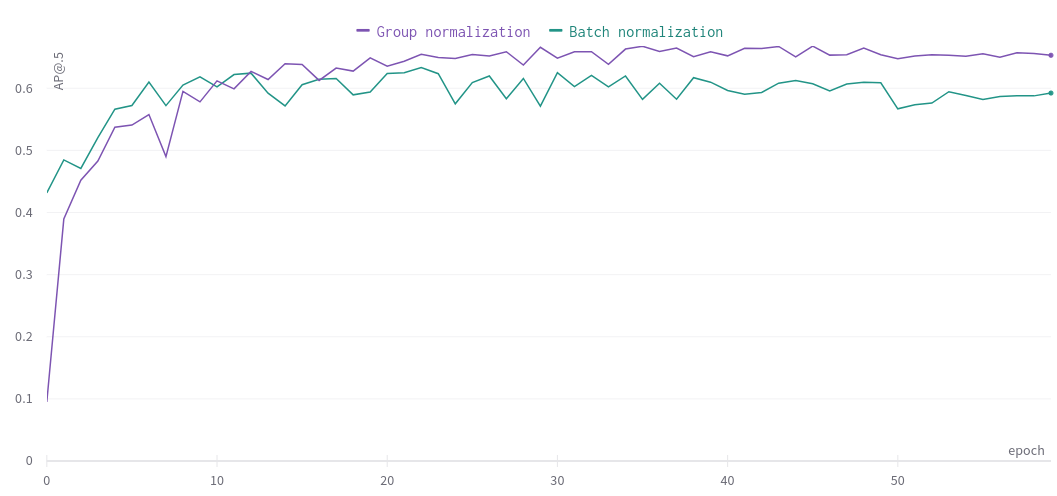
\includegraphics[width=\textwidth]{images/batch_norm_group_norm.png}
    \caption{Difference in $AP@.5$ among EfficientDet-D5 model with batch normalization and group normalization}
    \label{fig:batch_group_diff}
\end{figure}

\section{Model inspection}
\subsection{Size of backbone}
\begin{table}[H]
    \begin{tabular}{|c|c|c|c|c|}
        \hline
        Backbone & mean  & std    & max   & min   \\ \hline
        small    & 0.68  & 0.0197 & 0.651 & 0.697 \\ \hline
        medium   & 0.696 & 0.0126 & 0.669 & 0.719 \\ \hline
        large    & 0.703 & 0.0136 & 0.681 & 0.725 \\ \hline
    \end{tabular}
    \caption{Comparision of $AP.@5$ metric for different backbones of YOLOv5}
    \label{tab:backbone_comparison}
\end{table}

\subsection{Weight decay}

\begin{figure}[H]
    \begin{floatrow}[2]
        \ffigbox[\FBwidth]{
            \caption{$AP@.5$ of Faster-RCNN model with varying weight decay values. The metric is computed on validation part of the dataset during the course of triaing.  \label{fig:fasterrcnn_weight_decay}}
        }{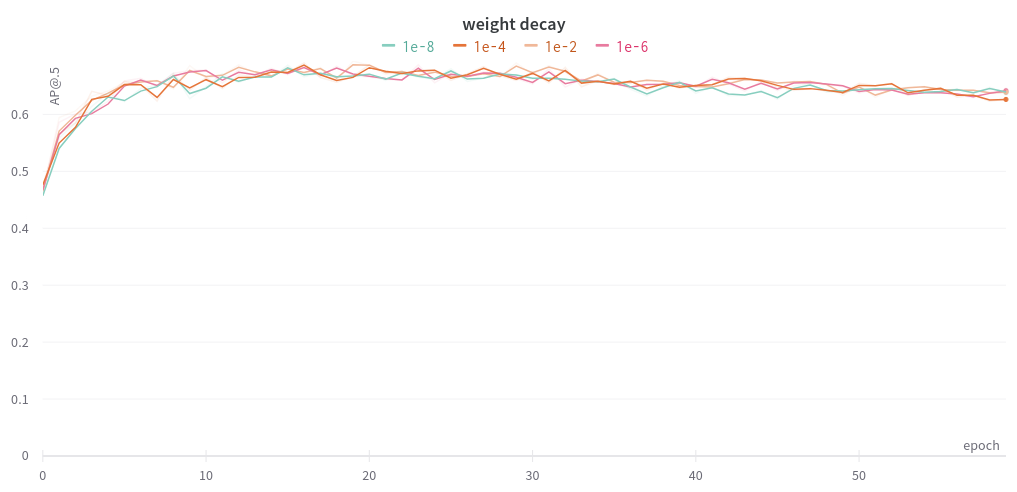
\includegraphics[width=\linewidth]{images/weight_decay_fasterrcnn.png}}
        \ffigbox[\FBwidth]{\caption{$AP@.5$ of YOLOv5 model with varying weight decay values. The metric is computed on validation part of the dataset during the course of triaing. \label{fig:yolo_weight_decay}}}
        { 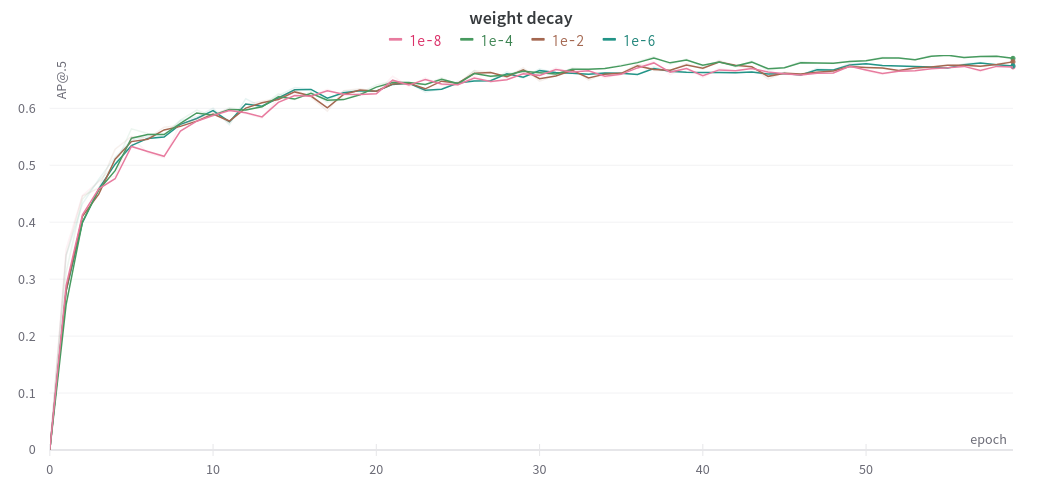
\includegraphics[width=\linewidth]{images/weight_decay_yolo.png} }
    \end{floatrow}
\end{figure}

\section{Ensembling}
\section{Hand-picked parameters}
\begin{table}[H]
    \begin{tabular}{|c|c|c|c|c|c|c|c|}
        \hline
        Ensembled models      & $AP$  & $AP@.3$ & $AP@.5$ & $AP@.75$ & $AP@.5_S$ & $AP@.5_M$ & $AP@.5_L$ \\ \hline
        RN-sw, YOLO-m, RN-res & 0.303 & 0.776   & 0.694   & 0.216    & 0.605     & 0.729     & 0.803     \\ \hline
        FR-R101, Y5-m, RN-sw  & 0.305 & 0.783   & 0.695   & 0.218    & 0.598     & 0.733     & 0.807     \\ \hline
    \end{tabular}
    \caption{WBF ensemble of multiple models, wehre we handpicked the parameters of the ensemble process. The models were trained on stage four dataset.}
    \label{tab:model_ensembling:handpicked}
\end{table}
\subsection{Grid search results}
The best hyper-parameters for a given ensemble method found by a grid search are in the table \ref{tab:ensemble_params:grid_search}. We omited from the table parameter $sigma$, used only in snms. Its optimal value, according to the grid search, was $0.8$.
Average precision of the models ensembled with parameters from table \ref{tab:ensemble_params:grid_search} are available in table \ref{tab:precision:grid_search} and average recall values are in the table \ref{tab:recall:grid_search}. Precison and recall values based on the confidence threshold, that maximizes F-score can be seen in table \ref{tab:ensembling_prf:grid_search}.

\begin{table}[H]
    \begin{tabular}{|c|c|c|c|c|c|c|}
        \hline
        Method & FRCNN-R50      & YOLOv5-m6      & RetN-swint     & FRCNN-R101     & $T$  \\ \hline
        nms    & 1              & 0.4            & 0.4            & 0.85           & 0.6  \\ \hline
        snms   & 1              & 0.12           & 0.12           & 0.12           & 0.7  \\ \hline
        nwm    & 0.85           & 0.25           & 0.70           & 0.85           & 0.45 \\ \hline
        wbf    & 1              & 0.4            & 0.85           & 0.85           & 0.65 \\ \hline
        wbf-A  & 0.94/0.77/0.84 & 0.31/0.47/0.31 & 0.98/0.85/0.88 & 0.72/0.69/0.91 & 0.64 \\ \hline
    \end{tabular}
    \caption{Hyper-parameter values of ensemble methods found by a grid-seach}
    \label{tab:ensemble_params:grid_search}
\end{table}


\begin{table}[h]
    \centering
    \begin{tabular}{|c|c|c|c|c|c|c|c|}
        \hline
        method & $AP$  & $AP@.3$ & $AP@.5$ & $AP@.75$ & $AP@.5_S$ & $AP@.5_M$ & $AP@.5_L$ \\ \hline
        nms    & 0.346 & 0.818   & 0.735   & 0.28     & 0.618     & 0.775     & 0.829     \\ \hline
        snms   & 0.348 & 0.807   & 0.722   & 0.295    & 0.609     & 0.758     & 0.819     \\ \hline
        nwm    & 0.364 & 0.829   & 0.759   & 0.302    & 0.641     & 0.802     & 0.854     \\ \hline
        wbf    & 0.378 & 0.832   & 0.77    & 0.323    & 0.663     & 0.807     & 0.875     \\ \hline
        wbf-A  & 0.376 & 0.832   & 0.768   & 0.318    & 0.651     & 0.806     & 0.875     \\ \hline
    \end{tabular}
    \caption{Average precision of models ensembled by parameters from table \ref{tab:ensemble_params:grid_search}}
    \label{tab:precision:grid_search}
\end{table}


\begin{table}[h]
    \centering
    \begin{tabular}{|c|c|c|c|c|c|c|c|}
        \hline
        method & $AR$  & $AR@.5_{10}$ & $AR@.5$ & $AR@.75$ & $AR@.5_S$ & $AR@.5_M$ & $AR@.5_L$ \\ \hline
        nms    & 0.546 & 0.91         & 0.971   & 0.522    & 0.949     & 0.98      & 0.98      \\ \hline
        snms   & 0.584 & 0.888        & 0.951   & 0.603    & 0.912     & 0.965     & 0.965     \\ \hline
        nwm    & 0.526 & 0.913        & 0.941   & 0.513    & 0.892     & 0.959     & 0.959     \\ \hline
        wbf    & 0.573 & 0.918        & 0.975   & 0.569    & 0.956     & 0.981     & 0.981     \\ \hline
        wbf-A  & 0.572 & 0.92         & 0.974   & 0.566    & 0.956     & 0.98      & 0.98      \\ \hline
    \end{tabular}
    \caption{Average recall of models ensembled by parameters from table \ref{tab:ensemble_params:grid_search}}
    \label{tab:recall:grid_search}
\end{table}


\begin{table}[h]
    \begin{tabular}{|c|c|c|c|c|}
        \hline
        Model - backbone & Precision & Recall & F-score & Confidence threshold \\ \hline
        nms              & 0.708     & 0.68   & 0.694   & 0.284                \\ \hline
        snms             & 0.679     & 0.7    & 0.689   & 0.489                \\ \hline
        nwm              & 0.713     & 0.71   & 0.712   & 0.792                \\ \hline
        wbf              & 0.732     & 0.7    & 0.715   & 0.594                \\ \hline
        wbf-A            & 0.745     & 0.69   & 0.716   & 0.201                \\ \hline
    \end{tabular}
    \caption{Precision, recall, and F-score based on the confidence threshold for different ensembling methods}
    \label{tab:ensembling_prf:grid_search}
\end{table}

\section{Assesing importance of different models}

\begin{table}[h]
    \centering
    \begin{tabular}{|c|c|c|c|c|c|c|c|}
        \hline
        Models     & $AP$  & $AP@.3$ & $AP@.5$ & $AP@.75$ & $AP@.5_S$ & $AP@.5_M$ & $AP@.5_L$ \\ \hline
        All        & 0.389 & 0.838   & 0.774   & 0.338    & 0.665     & 0.811     & 0.876     \\ \hline
        YOLOv5-mix & 0.379 & 0.819   & 0.75    & 0.34     & 0.636     & 0.79      & 0.84      \\ \hline
        YOLOv5-m   & 0.368 & 0.812   & 0.741   & 0.329    & 0.648     & 0.775     & 0.844     \\ \hline
    \end{tabular}
    \caption{Average precision of models ensembled by parameters from table \ref{tab:ensemble_params:grid_search}}
    \label{tab:precision:grid_search}
\end{table}


\begin{table}[h]
    \centering
    \begin{tabular}{|c|c|c|c|c|c|c|c|}
        \hline
        Models     & $AR$  & $AR@.5_{10}$ & $AR@.5$ & $AR@.75$ & $AR@.5_S$ & $AR@.5_M$ & $AR@.5_L$ \\ \hline
        All        & 0.586 & 0.917        & 0.978   & 0.582    & 0.946     & 0.991     & 0.991     \\ \hline
        YOLOv5-mix & 0.579 & 0.911        & 0.959   & 0.599    & 0.929     & 0.972     & 0.972     \\ \hline
        YOLOv5-m   & 0.562 & 0.906        & 0.949   & 0.572    & 0.909     & 0.964     & 0.964     \\ \hline
    \end{tabular}
    \caption{Average recall of models ensembled by parameters from table \ref{tab:ensemble_params:grid_search}}
    \label{tab:recall:grid_search}
\end{table}


\begin{table}[h]
    \begin{tabular}{|c|c|c|c|c|}
        \hline
        Models     & Precision & Recall & F-score & Confidence threshold \\ \hline
        All        & 0.751     & 0.7    & 0.725   & 0.294                \\ \hline
        YOLOv5-mix & 0.728     & 0.69   & 0.708   & 0.241                \\ \hline
        YOLOv5-m   & 0.726     & 0.67   & 0.697   & 0.272                \\ \hline
    \end{tabular}
    \caption{Precision, recall, and F-score based on the confidence threshold for different ensembling methods}
    \label{tab:ensembling_prf:grid_search}
\end{table}

\section{Dental retorations segmentation}
\subsection{Non-deeplearning approach}
Hyper-parameters ensuring the best performance on validation part of the datset are in table \ref{tab:nondl_restorations:best_params}. Performance of the pipelie on test dataset given the parameters in table \ref{tab:nondl_restorations:best_params} can be seen in table \ref{tab:nondl_results}.

\begin{table}[H]
    \begin{tabular}{|c|c|c|c|}
        \hline
        Hyper-parameter & Adaptive mean & Adaptive Gaussian & Otsu's \\ \hline
        $K_t$           & 71            & x                 & -      \\ \hline
        $T$             & 15            & x                 & -      \\ \hline
        $K_d$           & 41            & x                 & 61     \\ \hline
        $K_o$           & 31            & x                 & 36     \\ \hline
        $K_b$           & -             & x                 & 21     \\ \hline
    \end{tabular}
    \caption{Best hyper-parameters for non-deeplerning pipeline}
    \label{tab:nondl_restorations:best_params}
\end{table}


\begin{table}[H]
    \centering
    \begin{tabular}{|c|c|c|}
        \hline
        Model               & Dice  & IOU   \\ \hline
        Adaptive mean       & 0.364 & 0.314 \\ \hline
        Adaptive Gaussian   & 0.102 & 0.088 \\ \hline
        Otus's thresholding & 0.102 & 0.088 \\ \hline
    \end{tabular}
    \caption{Results of non-deeplerning approach to dental resotrations segmentation given the hyper-parameters in table \ref{tab:nondl_restorations:best_params}}
    \label{tab:nondl_results}
\end{table}



\subsection{U-Net}

\begin{figure}[H]
    \centering
    \begin{subfigure}[b]{\textwidth}
        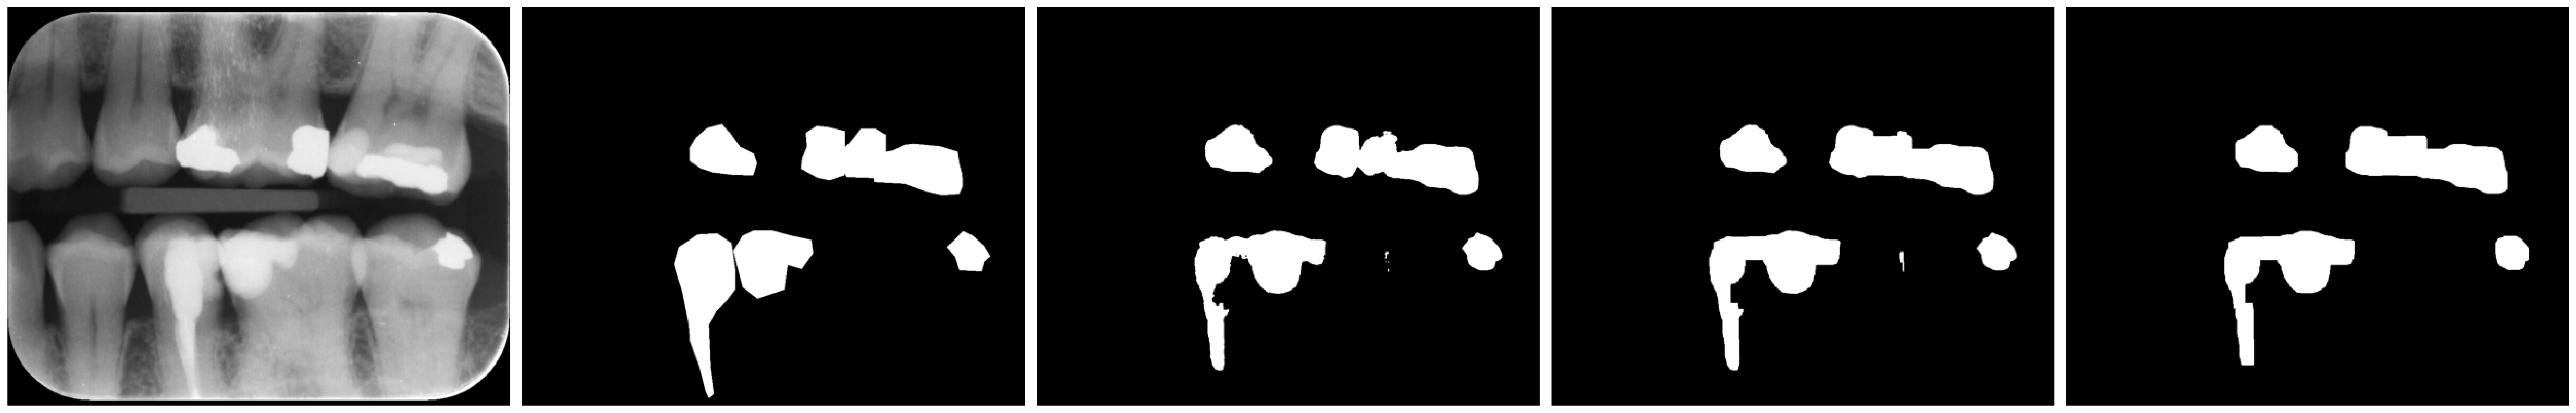
\includegraphics[width=1\linewidth]{images/unet_1_img_12.pdf}
        \caption{Baseline U-Net model}
    \end{subfigure}

    \begin{subfigure}[b]{\textwidth}
        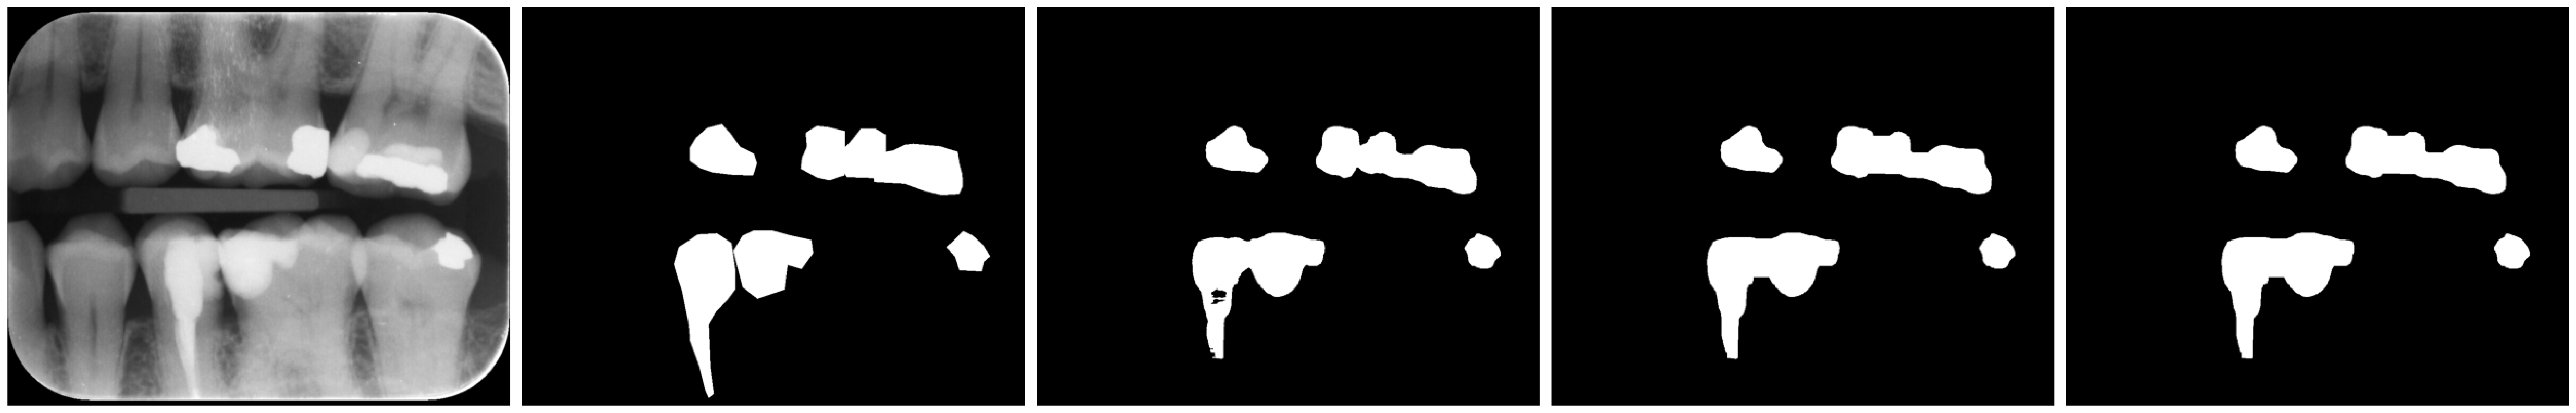
\includegraphics[width=1\linewidth]{images/unet_2_img_12.pdf}
        \caption{Imrpoved U-Net model}
    \end{subfigure}
    \caption{From the left: X-ray image, ground-truth pixel mask, output of the model, output processed by morphological opening, output post-processed by morphological opening and closing.}
\end{figure}

\begin{figure}[H]
    \centering
    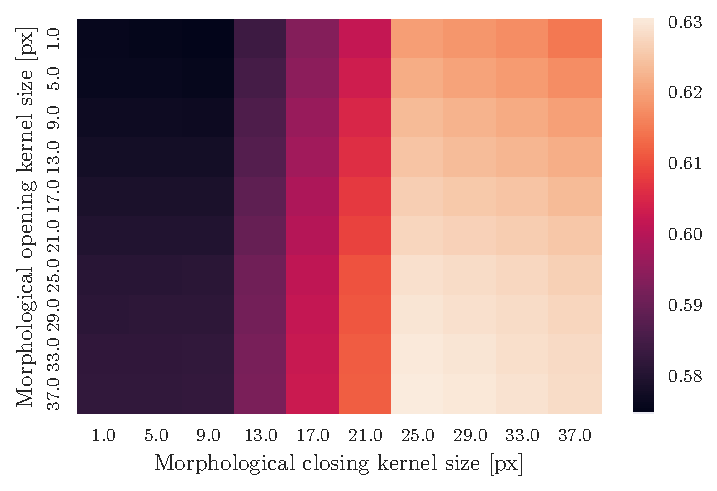
\includegraphics[]{images/heatmap_of_unetpostproc_search.pdf}
    \caption{Value of IOU metric based on the size of kernels $K_o$, $K_c$ in morphological operations, that were used for post-processing}
    \label{fig:heatmap_postprocess}
\end{figure}

\begin{table}[H]
    \centering
    \begin{tabular}{|c|c|c|}
        \hline
        Parameter      & $K_o$ & $K_c$ \\ \hline
        U-Net          & 37    & 25    \\ \hline
        U-Net improved & 33    & 5     \\ \hline
    \end{tabular}
\end{table}

\begin{table}[H]
    \centering
    \begin{tabular}{|c|c|c|}
        \hline
        Model      & Dice  & IOU   \\ \hline
        U-Net-B    & 0.663 & 0.575 \\ \hline
        U-Net-B-PP & 0.714 & 0.623 \\ \hline
        U-Net-I    & 0.747 & 0.662 \\ \hline
        U-Net-I-PP & 0.760 & 0.676 \\ \hline
    \end{tabular}
    \caption{Results of U-Net models}
\end{table}

